\chapter{Collision Avoidance}
\label{chapter:collisionavoidance}
In the following chapter, we introduce our proposed method for collision avoidance. We implemented an inequality task inside the SoT, which is placed as a high priority task. This task handles all collisions, but still restricts the execution of lower priority tasks as little as possible. The collision avoidance task, introduced in the following, is based on three major concepts. 
\begin{enumerate}
\item Closest point pair calculation between two collision objects
\item Damping the velocity along the normal vector, spanning from the closest point pair
\item Calculating the Jacobian for every closest point
\end{enumerate}
\section{Closest Point Calculation}\label{sec:closestpoints}
Closest point pairs are used in various algorithms for collision avoidance \cite{conf/icra/DietrichWTAH11}\cite{Kanehiro-RSS08}. Hereby, a Gilbert-Johnson-Keerthi (GJK) approach is frequently used to compute the proximity and closest points for collision detection \cite{VandenBergen:1999:FRG:334709.334711}. It is easy to understand, that preventing the closest points of two colliding objects is sufficient enough for avoiding the complete object to collide. However, this is constrained with the condition, that there is always one unique pair of closest points \cite{conf/humanoids/EscandeMK07}. 
\clearpage
\subsection{Collision Geometry - Mesh}
Most common robots come along with a description of their collision geometry. In order to make the collision geometry as accurate as possible, polygon meshes are widely used to represent the geometry of the robot. The interested reader is referred to \cite{Tobler_amesh} for more information.

Although the calculation between two meshes might fulfill the requirement of having a unique point pair between two collision objects, severe discontinuities occur inside a two dimensional space. Depending on the alignment of the vertices inside the mesh, the closest points can jump in $X$ as well as $Y$ direction, when two meshes appear to be coplanar to each other. In this case, there is ambiguity in the placement of the two points. Figure \ref{figclosestpointmesh} illustrates this behavior. The discontinuities shown here are linearly propagated to the velocity of the moving body part, which finally results in a heavy jump of velocity.\\
The discontinuities occur quite frequently in two aspects. The points can vary inside one pair of vertices as illustrated in figure \ref{figclosestpointmesh}. Additionally, depending on the shape of the mesh, multiple vertices can be projected towards the same pose, respectively a high number of normal vectors of each vertices (see figure \ref{figmeshambiguity}). This makes a closest point calculation for meshes infeasible.  

\begin{figure}[h!]
  \centering
    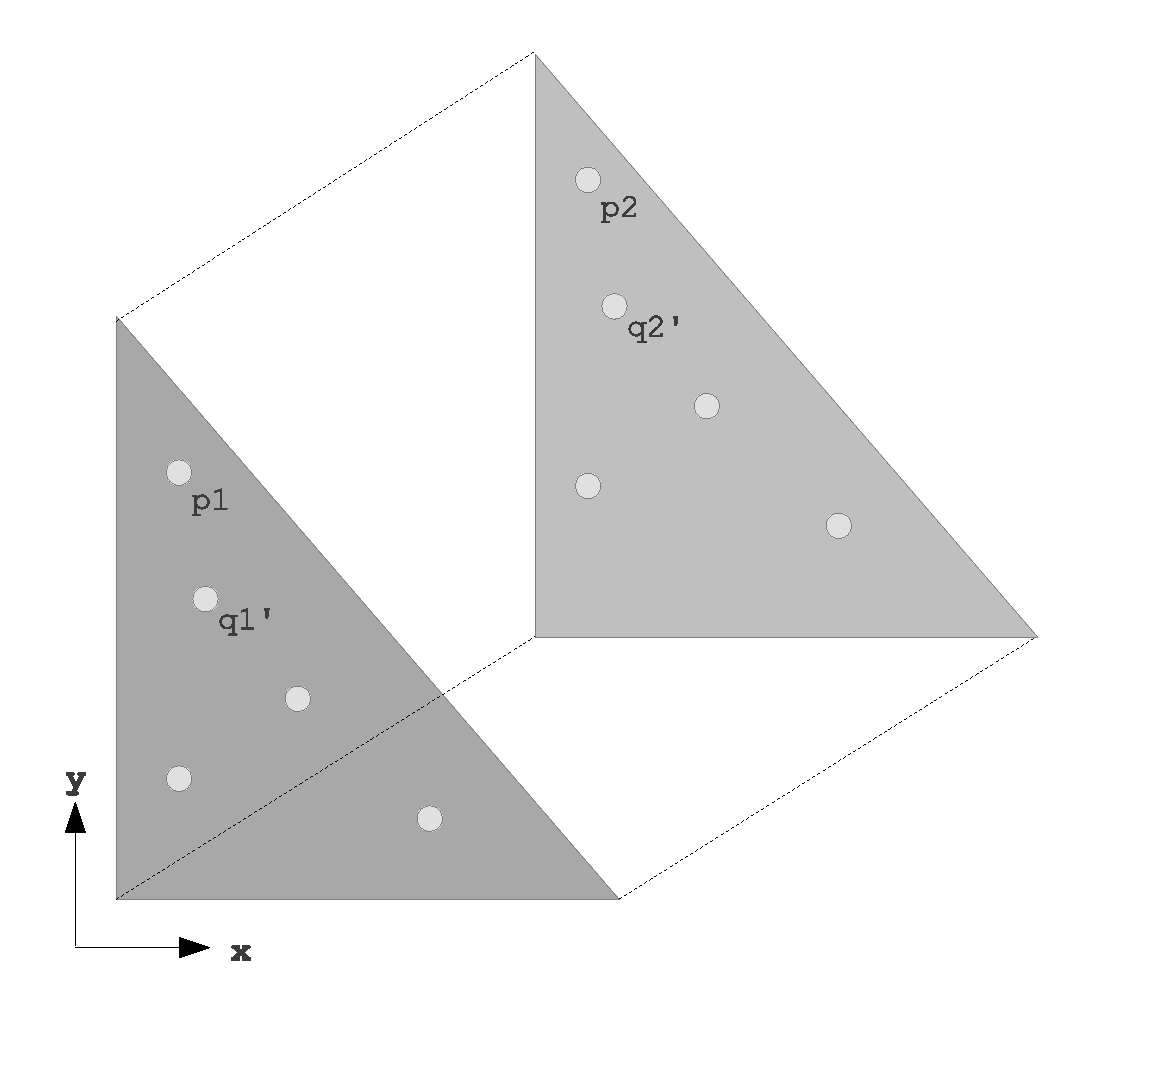
\includegraphics[width=0.6\textwidth]{../figures/closestpointmesh.eps}
    \caption{Discontinuity of closest point calculation for two vertices inside meshes. Parallelism of two vertices produces an ambiguity of the point pair. As depicted here, multiple solutions exists such as $p1$, $p2$ as well as $p1'$, $q2'$.}
    \label{figclosestpointmesh}
\end{figure}

\begin{figure}[h!]
  \centering
    \includegraphics[width=0.3\textwidth]{../figures/mesh_head.png}
    \includegraphics[width=0.3\textwidth]{../figures/mesh_torso.png}
    \includegraphics[width=0.3\textwidth]{../figures/mesh_base.png}
    \caption{Example for high resolution meshes. It can be easily seen, that a high number of the same normal vectors exist on the meshes. This makes a parallel configuration quite likely and the closest points can jump discontinuously.}
    \label{figmeshambiguity}
\end{figure}

\subsection{Collision Geometry - Capsule}\label{subsec:capsulecalculation}
To overcome the discontinuities mentioned in the previous section, we implemented a complete capsule decomposition for this work. A capsule describes a 3-dimensional geometry object, which consists of a cylinder along a 3-dimensional main axis and a length $l$ and radius $r$. In difference to the cylinder, each capsule comprises a half sphere at both ends of the cylinder. Since capsules are pseudo convex collision geometries, the probability of discontinuities is relatively low. There exists exactly one configuration, where ambiguity can occur. Essentially this happens, when the main axis of both capsules are parallel. Figure \ref{capsulecapsule} expresses two possible configuration for closest point pairs. It can be seen that as long as the main axis are not parallel aligned, both capsules can be treated as strictly convex objects. This convexity results in a unique point pair. \\
Furthermore, a capsule decomposition allows a smoother continuous trajectory compared to mesh to mesh calculation. In the case of parallel main axis, the dimension of possible discontinuities compared to meshes is limited to one dimension along the main-axis 
\begin{equation}
	\vec{p_i} + l_i  \vec{n} \quad i \in [CP_1,CP_2], l \in \mathbb{R}, \vec{n} \in \mathbb{R}^3
\end{equation}
where $p_i$ describes the start point of the cylinder with $z=0$, $l_i$ the length of the capsule and $n$ the orientation of the main axis. Note that in this specific case, we do not differentiate $n_{C1}$ and $n_{C2}$ as both capsules are considered to be parallel and the $z$ component is pointing along the axis. 
\newpage
Given this definition, the distance of possible discontinuities can be formulated as
\begin{eqnarray}
	\vec{p_1}	 + l_1  \vec{n} &=& \vec{p_2} + l_2  \vec{n} \\
	\vec{p_1} + l_1 \vec{n} - (\vec{p_2} + l_2 \vec{n}) &=& 0 \\
	(p_{z1} + l_1) &-& (p_{z2} + l_2) \label{eqnz}
\end{eqnarray}

where in equation \ref{eqnz}, only the $Z$ component has to be considered. $X$ and $Y$ are equal, since the two capsules are parallel.
\begin{figure}[h!]
\centering     %%% not \center
\subfigure[Unique solution]{\label{fig:capsulea}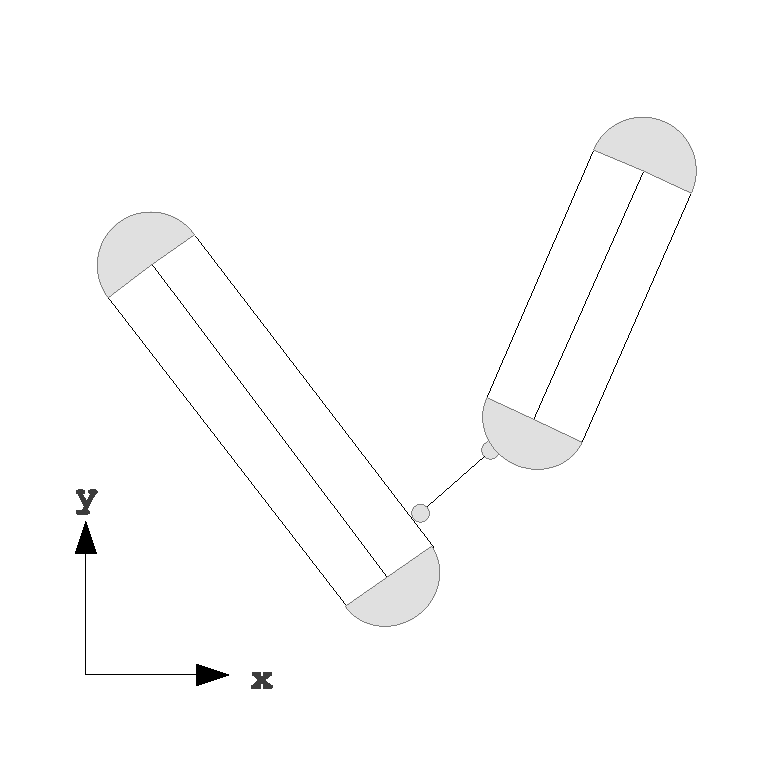
\includegraphics[width=0.48\textwidth]{../figures/capsulecapsule.eps}}
\subfigure[Parallel configuration]{\label{fig:capsuleb}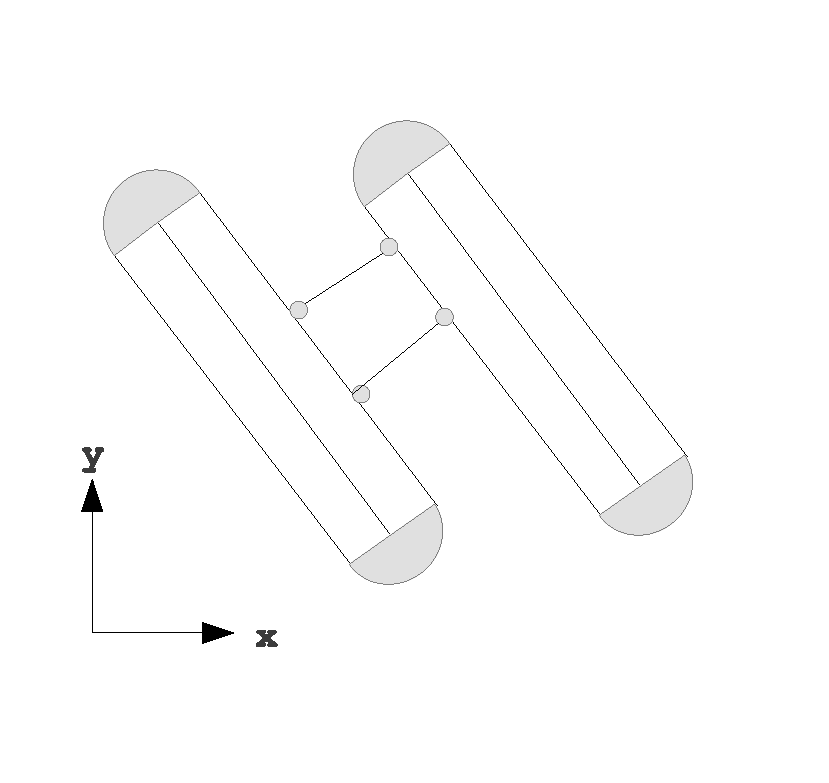
\includegraphics[width=0.48\textwidth]{../figures/capsulecapsule_parallel.eps}}
\caption{a) shows a unique solution of a closest point pair. b) shows two capsules in a parallel configuration. Note that in comparison to meshes, the ambiguity spans only along the main axis of the capsules. In a continuous motion of both capsules, these discontinuities are from no further importance, because the probability is rather low.} 
\label{capsulecapsule}
\end{figure}

\subsection{Closest Point Pair for Capsule-Capsule}
We concluded in the previous section \ref{subsec:capsulecalculation}, that a capsule decomposition of collision objects is to be preferred over meshes, because of the reduction of discontinuities. In this section, we describe the algorithm for the actual computation of the closest point pair. The presented algorithm is a derivative of the closest points based on two line segments as it is verbosely described in \cite{Ericson:2004:RCD:1121584}. Since we define a capsule to be a finite line segment in $\mathbb{R}^3$ with spatial radius information, we can modify the line segment algorithm to fit the calculated point on the surface of the capsule.

\subsubsection*{Infinite Lines}
We start our calculation by looking at the closest point calculation of two lines. According to \cite{Ericson:2004:RCD:1121584}, we formulate a line pair in $\mathbb{R}^3$ as follows.
\begin{eqnarray} \label{eqnline}
LS_1(s) &=& \vec{p_1} + s\vec{d_1} \notag\\
LS_2(t) &=& \vec{p_2} + t\vec{d_2}\notag \\
\textit{where } && \vec{d_i} = \vec{q_i} - \vec{p_i}
\end{eqnarray}
The start- and endpoint are declared as $\vec{p}$ and $\vec{q}$ in $\mathbb{R}^3$, respectively. $\vec{d}$ indicates the directional vector between $\vec{p}$ and $\vec{q}$. We find a solution for a closest point pair $s,t$, whose vector 
\begin{equation}\label{lsvec}
\vec{v}(s,t) = LS1-LS2
\end{equation}
gets minimal in length. Example is given in figure \ref{fig:lsa}.

The shortest vector $\vec{v}(s,t)$ can be examined as the scalar product of the two lines. Since the vector has to be perpendicular to both lines, the following equation system for the scalar product can be formulated:
\begin{eqnarray}
\vec{d_1} \vec{v}(s,t)&=& 0  \notag \\
\vec{d_2} \vec{v}(s,t)&=& 0  
\end{eqnarray}
we solve this equation system by substituting $\vec{v}(s,t)$ with the definition of \ref{lsvec}. Further steps are invoked:
\begin{eqnarray}
\vec{d_1} (LS_1-LS_2) &=& \vec{d_1} ((\vec{p_1}-\vec{p_2}+s\vec{d_1}- t\vec{d_2}) = 0  \notag \\
\vec{d_2} (LS_1-LS_2) &=& \vec{d_2} ((\vec{p_1}-\vec{p_2}+s\vec{d_1}- t\vec{d_2}) = 0
\end{eqnarray}
\begin{eqnarray}
(\vec{d_1}\vec{d_1})s - (\vec{d_1}\vec{d_2})t &=& -\vec{d_1}k \notag \\
(\vec{d_1}\vec{d_2})s - (\vec{d_2}\vec{d_2})t &=& -\vec{d_2}k
\end{eqnarray}
where $k= \vec{p_1}-\vec{p_2}$.
Using Cramer's rule \cite{cramer1750introduction} for solving 2x2 linear equation system finally yields the solution for $s$ and $t$:
\begin{eqnarray}
s&=& (b f - c e) / d \notag \\
t &=& (a f - b e) / d 
\end{eqnarray}
where $a = \vec{d_1^2}, b = \vec{d_1 d_2}, c = \vec{d_2^2}, e = \vec{d_1}k, f = \vec{d_2}k, d=  \vec{d_1^2}\vec{d_2^2}- (\vec{d_1 d_2})^2$ \\
Special care has to be taken in case $d=0$, which means that both lines are parallel.

\subsubsection*{Line Segments}
Compared to lines, line segments are of finite length. This necessitates a case differentiation of the spatial pose relation between two line segments. For this, we simply restrict the length along the directional vector in the range from 0 to 1.
Thus, we modify equation \ref{eqnline} according to:
\begin{equation}
LS_i(s) = \vec{p_i} + s\vec{d_i} \quad \textit{where } \vec{d_i} = \vec{q_i} - \vec{p_i}, 0 \leq s \leq 1
\end{equation}

With this formulation, we cannot apply the solution used in the previous section, as there might not be a perpendicular vector $v$ for all configurations. This situation happens, when at least one line segments lies outside the line segment of the other. In the following, we examine four different cases as illustrated in figure \ref{figlinesegments}.

When a configuration occurs as shown in figure \ref{fig:lsa}, we can apply the solutions as if the two line segments were infinite lines. When one closest point $CP_1$ lies outside its line segments, yet inside the segment of the corresponding other line, we can clamp $CP_1$ to the end of the line segment and compute the minimum distance to $LS_2$, in order to find $CP_2$. This behavior is illustrated in figure \ref{fig:lsb}. In case both closest points lie outside the corresponding line segments (see figure \ref{fig:lsc}, the procedure of \ref{fig:lsb} has to be repeated twice. We first clamp $CP_1$ to the end point and calculate $\hat{CP_2}$ . As depicted in figure \ref{fig:lsc}, this point lies outside $LS_2$ and results in a invalid point. To overcome this issue, we clamp $\hat{CP_2}$ to the endpoint of $LS_2$ and repeat the computation now inverse. We recompute $CP_1$ and see that this lies now inside $LS_1$. Figure \ref{fig:lsd} illustrates the very extreme, where both points are clamped to their respective end points.

\begin{figure}[h!]
\centering     %%% not \center
\subfigure[]{\label{fig:lsa}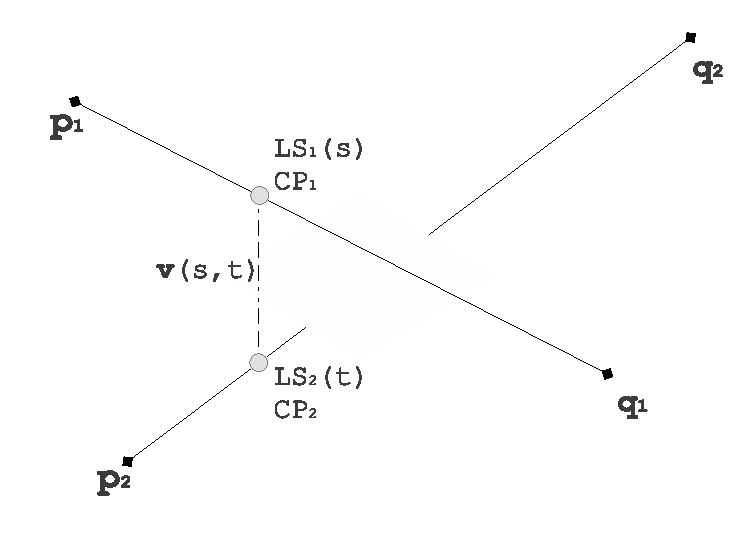
\includegraphics[width=0.4\textwidth]{../figures/linesegments1.eps}}
\subfigure[]{\label{fig:lsb}\includegraphics[width=0.4\textwidth]{../figures/linesegments2.eps}}
\subfigure[]{\label{fig:lsc}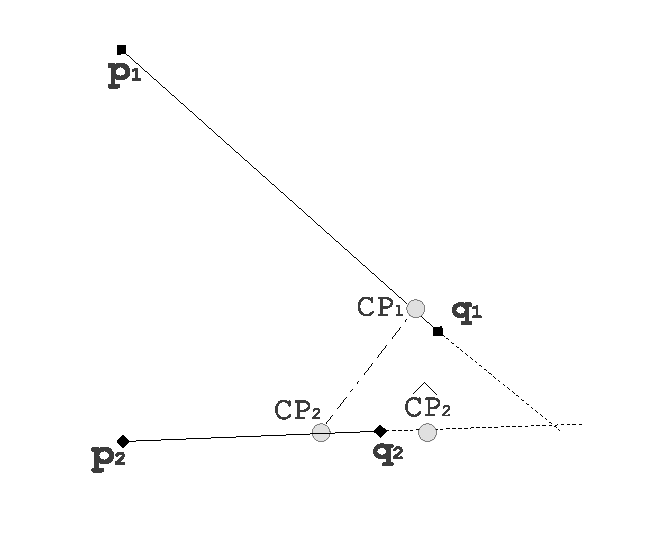
\includegraphics[width=0.4\textwidth]{../figures/linesegments3.eps}}
\subfigure[]{\label{fig:lsd}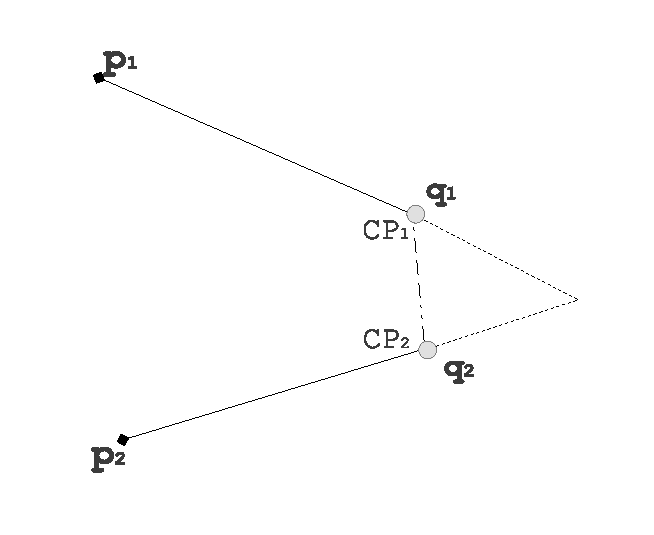
\includegraphics[width=0.4\textwidth]{../figures/linesegments4.eps}}
\caption{Relative spatial poses between two line segments. a) closest point pair lies inside both segments. b) endpoint $q_1$ is a closest point, the second closest point lies on the line segment. c) both closest points would lie outside their corresponding line segments. Here, a recursive clamping has to be implemented. d) both ending points $p_1$ and $p_2$ are closest points. } 
\label{figlinesegments}
\end{figure}

Finally, the solving process is separated in two parts. Firstly, we have to decide for the clamping of the respective points. This case study is examined according to the above description. Secondly, once the points are clamped, we can mathematically solve for the closest points.\\
We have a point $LS_2$ lying on the second segment:
\begin{equation}
LS_2(t) = \vec{P_2} + t\vec{d_2}
\end{equation}
The first point $LS_1$ is found via:
\begin{eqnarray}
LS_1(s) &=& \vec{P_1} + s\vec{d_1} \notag \\
s &=& (LS_2(t) -  \vec{P_1})\vec{d_1} / \vec{d_1}\vec{d_1} \notag \\
  &=& (\vec{P_2}+ t\vec{d_2}-\vec{p_1}\vec{d_1}/ \vec{d_1}\vec{d_1}
\end{eqnarray}
Obviously, this formulation also determines $LS_2$, given $LS_1$.

\subsubsection*{Capsules}
In the beginning of this chapter, we defined a capsule as a line segment with a spatial radius. For the closest point computation on two capsules, we enhance the algorithm for line segments slightly to project the closest on the border of the capsule.\\
As we know the two closest points $\hat{\vec{CP_1}}$ and $\hat{\vec{CP_2}}$ of the two respective line segments, we can use this information to calculate the directional vector between them. The projection is to the border of the capsule is done by shifting the closest points along this vector by the radius. Figure \ref{fig:capsulevec} shows this projection.
\begin{figure}[h!]
  \centering
    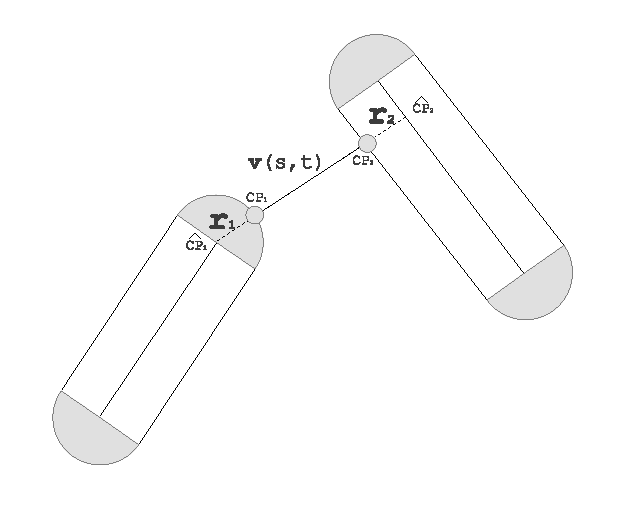
\includegraphics[width=0.7\textwidth]{../figures/capsulecapsule_vector.eps}
    \caption{Projection of the two closest points $\hat{\vec{CP_1}}$ and $\hat{\vec{CP_2}}$ to the border of the capsule. $\vec{v(s,t)}$ describes the directional vector along which the projection is done with length $r_i$.}
    \label{fig:capsulevec}
\end{figure}

We can formulate this solution, given the two closest points $\hat{\vec{CP_1}}, \hat{\vec{CP_2}}$. We calculate the vector $\vec{v}$:
\begin{equation}
\vec{v} = \hat{\vec{CP_2}}-\hat{\vec{CP_1}}
\end{equation}
The shifting is done via:
\begin{eqnarray}
\vec{CP_1} &=& \hat{\vec{CP_2}} + r_1 \vec{v} \notag \\
\vec{CP_1} &=& \hat{\vec{CP_1}} - r_2 \vec{v} \notag \\
\end{eqnarray}

\section{Velocity Damping}\label{sec:velocitydamping}
In section \ref{chapter:soth} we pointed out that every task has to be designed in the form of 
\begin{equation}
\vec{Ax-b} \quad  \vec{A} \in \mathbb{R}^{m \times n}, \vec{x} , \vec{b} \in \mathbb{R}^{m}
\end{equation}
In this section, we introduce the task formulation for collision avoidance. The collision avoidance task restricts any possible movement along the unitvector between the closest point pair, we calculated in the previous section. The presented approach was firstly introduced in \cite{Faverjon87alocal} and reformulated inside the SoT \cite{Kanehiro-RSS08}. 
As we have seen in equation \ref{eqn:ikleastsquare}, controlling a body part in cartesian space corresponds to the IK formulation  
\begin{equation}\label{gototask}
\vec{J(p,q) \dot{q} - \dot{x}} \quad  \vec{J} \in \mathbb{R}^{m \times n}, \vec{\dot{q}, \dot{x}} \in \mathbb{R}^{n}
\end{equation}
where $\vec{J(p,q)}$ names the Jacobian of point $\vec{p}$ at joint vector position $\vec{q}$, the resulting joint velocities $\vec{\dot{x}}$ and the cartesian goal velocity. This formulation solves for all available DoF inside the hierarchy. In order to restrict the solution for one direction, we modify the above formulation in two aspects.
\begin{itemize}
	\item The Jacobian is projected onto the unitvector spanned by the closest point pair
	\item The task is formulated as an inequality, which introduces a lower boundary for the proximity (distance) of the two body parts
\end{itemize}

\subsection{Jacobian Projection}
The configuration setup according to \cite{Faverjon87alocal} is depicted in figure \ref{figcapsuledistance}. The figure shows a close up view of a capsule pair, with closest points $\vec{p_1}$ and $\vec{p_2}$. Hereby, we consider the point $\vec{p_1}$ as the moving body part, whereas $\vec{p_2}$ is meant to be fixed\footnote{We establish the task with this convention of $\vec{p_2}$ being fixed in space. However, the implementation necessarily allows both points to be moving.} in $\mathbb{R}^3$ as a collision object. The unitvector $\vec{n}$ is defined as
\begin{equation}
	\vec{n} = \vec{\frac{p_1-p_2}{\Vert p_1 - p_2 \Vert}}
\end{equation}

The distance is computed according to the euclidean L2-Norm:
\begin{equation}
	d = \Vert \vec{p_1-p_2} \Vert = \sqrt[2]{(\vec{p_1-p_2})^2}
\end{equation}

\begin{figure}[h!]
  \centering
    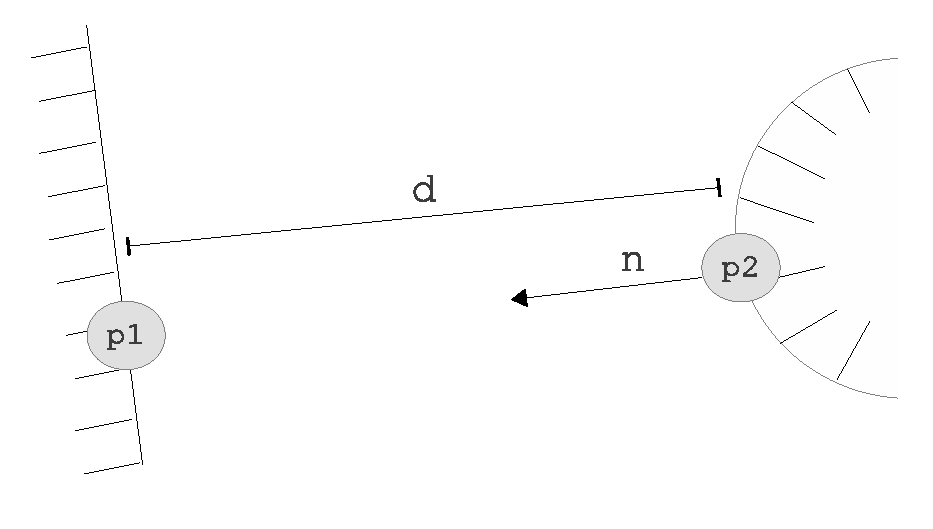
\includegraphics[width=0.8\textwidth]{../figures/capsuledistance.eps}
    \caption{A close up view of two capsules. The unitvector $n$ is pointing from $p_2$ to $p_1$. The distance $d$ corresponds to the euclidean L2-norm of $p_1$ and $p_2$.}
    \label{figcapsuledistance}
\end{figure}

To begin with, we modify the task definition in equation \ref{gototask} to restrict only the projection along $n$. Thus, the new task formulation becomes
\begin{equation}\label{gototaskn}
\vec{n^TJ(p_1,q) \dot{q} - \dot{x}} \quad ,\vec{n} \in \mathbb{R}^m, \vec{J} \in \mathbb{R}^{m \times n}, \vec{\dot{q}} , \vec{\dot{x}} \in \mathbb{R}^{m}
\end{equation}
where $\vec{n^T}$ describes the scalar product of $\vec{n}$ and $\vec{J}$. Informally spoken, we can treat the scalar product as the projection of the Jacobian onto the unitvector pointing towards the collision center. Note that we annotate the Jacobian parameters with respect to $p_1$. With this, we indicate, that the Jacobian has to be calculated in respect to the closest point $p_1$. The next section \ref{sec:jacobian} gives a more detailed examination on it.

\newpage
\subsection{Inequality Formulation}
To avoid a possible collision between two capsules, we have to ensure that the distance between them will always be larger than zero. To guarantee a minimal distance threshold, we transform the task in equation \ref{gototaskn} into an inequality constraint. Furthermore, we introduce a lower bound with respect to the actual distance. The outer circle in figure \ref{figcapsuledistanceds} represents this lower bound, where the minimal proximity of the point pair $\vec{p_1}$,$\vec{p_2}$ has to be larger than $d_s$.
\begin{figure}[h!]
  \centering
    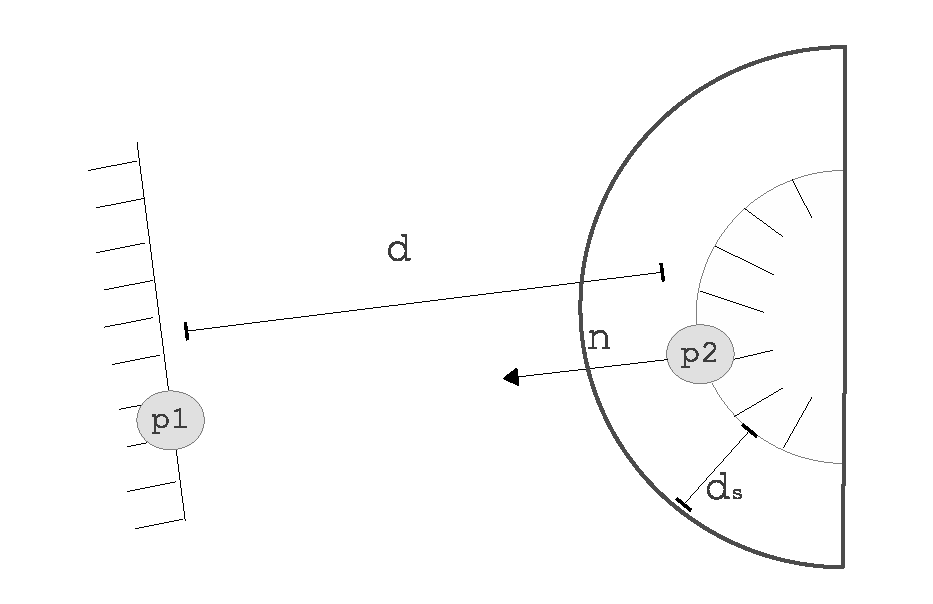
\includegraphics[width=0.8\textwidth]{../figures/capsuledistanceds.eps}
    \caption{To ensure a minimal proximity between two capsules, a security distance $d_s$ is introduced. The closest point $\vec{p_1}$ has to be outside the distance zone.}
    \label{figcapsuledistanceds}
\end{figure}
The solution space for this inequality task is formulated in respect to the current distance $d$. Thus, the equation \ref{gototaskn} evolves to an inequality constraint
\begin{equation}\label{gototaskds}
\vec{n}^T\vec{J(p_1,q)} \vec{\dot{q}} \geq - \epsilon \frac{d - ds}{\Delta t}\quad , \epsilon, d, d_s, \Delta t \in \mathbb{R}
\end{equation}
where $d-d_s$ calculates the distance along $\vec{n}$. The velocity towards the collision center undergoes a damped course, hence the name velocity damping.
We stress out the $\Delta t$ in equation \ref{gototaskds} to demonstrate the calculation in the velocity domain. In the implementation although, this value is not available as a parameter, since the control gain value $\epsilon$ has to be tuned for each application, which may compensate for $\Delta t$. \\
We can see that the velocity converges to zero with decreasing proximity between the closest point pair.
\begin{equation}
\lim\limits_{d \rightarrow d_s}{- \epsilon\frac{d - ds}{\Delta t} = 0}
\end{equation}
\newpage
We can now formulate the overall optimization problem as a task space formulation where a position $\vec{x_d}$ is specified as a goal position and $\vec{x}$ the current cartesian position. The optimization of this task is now subject to the velocity damping constraint developed in this section. The verbose formulation of the QP looks as the following:
\begin{eqnarray}
\underset{\vec{\dot{q}}}{\text{min}} \rightarrow \Vert \vec{J(p_x,q) \dot{q} - \dot{x}} \Vert^2  \notag \\
\underset{\vec{\dot{q}}}{\text{min}} \rightarrow \Vert \vec{J(p_x,q) \dot{q}} - \frac{(\vec{x-x_d})}{\Delta t} \Vert^2  \\
\text{subject to} \quad \vec{n}^T\vec{J(p_1,q)} \vec{\dot{q}} \geq - \epsilon \frac{d - ds}{\Delta t} \label{eqn:taskdampconstraint}
\end{eqnarray}

One note to the above formulation: It might look counter-intuitive at a first glance to design the task like this. One would presume a twist in the directions of $\vec{n}$ as well as the preceding minus sign in equation \ref{gototaskds}. It is more intuitive to assume $\vec{n}$ to point from $\vec{p_1}$ to $\vec{p_2}$. This modulation comes directly from the architecture of the hierarchical solver as a first-order control system. We review again the derivation of a task in cartesian space, which is depicted in the diagram \ref{fig:ikcontrolloop}.
\begin{eqnarray}
\vec{J(q)\dot{q}} &=& \vec{\dot{x}} \notag \\
\vec{J(q)\dot{q}} &=& K \frac{\vec{x - x_d}}{\Delta t} \label{eqnplus}  \\
\vec{J(q)\dot{q}} &=& -K \frac{\vec{x_d - x}}{\Delta t} \label{eqnminus}  \\
\vec{\dot{x}} &\equiv& - \hat{K} \vec{x_e} \quad, \text{where } \hat{K}= \frac{k}{\Delta t} \label{eqnfirstorder}
\end{eqnarray}
We can see from the above formulation that between equation \ref{eqnplus} and equation \ref{eqnminus} the sign changed as the formulation of the error between $\vec{x}$ and $\vec{x_d}$ swapped. Finally, \ref{eqnfirstorder} results in a common first-order control system formulation. The velocity damping task obeys this formulation.

\subsection{Integration into Hierarchy Solver}
The QP formulation represents an example for one collision pair. Equation \ref{eqn:taskdampconstraint} describes an inequality constraint for one closest point pair $\vec{p_1}$,$\vec{p_2}$ and the according distance $d$.\\
Obviously regarding the self-collision avoidance, we have to extend this to integrate multiple velocity damping constraints.
Depending on the application, it might be important on which level these inequality constraints are placed inside the solver hierarchy. This further depends which relative level the damping constraints have to each other inside the hierarchy. We can consider two cases:

\begin{itemize}
\item Constraints are on the same level
\item Constraints are on different level
\end{itemize}

\subsubsection*{Same Level}
Looking at self-collision avoidance, it is necessary that all collision pairs are on an equal level inside the solver hierarchy. This comes with no surprise, as one would expect the left arm being equally treated as the right arm in terms of avoiding self-collision. \\
To achieve this, we can concatenate the formulation given in \ref{eqn:taskdampconstraint}. For multiple collision points inside one task, the formulation evolves to:
\begin{equation}
\vec{n_i}^T\vec{J(p_{1,i},q)} \vec{\dot{q}} \geq - \epsilon_i \frac{d_i - d_{s,i}}{\Delta t} \quad \forall i \in \textit{\{1, \dots ,k\} }
\end{equation}
where $i$ iterates over all $k$ available collision pairs, which are considered to be on the same level. Written in matrix notation, this yields to

\begin{eqnarray}
\begin{pmatrix}
 \vec{n_1}^T\vec{J_1} \\
 \vdots \\[0.5em]
 \vec{n_k}^T\vec{J_k}
\end{pmatrix} 
 \vec{\dot{q}} &\geq &
 \begin{pmatrix}
 \vec{\dot{d_1}} \\
 \vdots \\[0.5em]
 \vec{\dot{d_k}}
\end{pmatrix} \notag \\
\vec{N} \vec{\dot{q}} &\geq & \vec{D} \notag \\
\textit{where } \vec{J_i} &=& \vec{J(p_{1,i},q)} \notag \\
\textit{and } \vec{\dot{d_i}} &=& \frac{d_i - d_{s,i}}{\Delta t}
\end{eqnarray}
Again the complete QP respecting all constraints at the same level yields:
\begin{eqnarray}
\underset{\vec{\dot{q}}}{\text{min}} \rightarrow \Vert \vec{J(p_x,q) \dot{q} - \dot{x}} \Vert^2  \notag \\
\text{subject to} \quad \vec{N}\vec{\dot{q}} \geq \vec{D} \label{eqn:taskdampconstraintsamelevel}
\end{eqnarray}


\subsubsection*{Different Level}
There may be applications, where multiple hierarchy steps are feasible. One could think of setting priority to self-collision avoidance over external collision avoidance. In this case, no further modifications have to be implemented for the task itself. This approach can simply be realized by stacking the two instances of the velocity damping task on top of each other.

\section{Jacobian Calculation for Closest Point}
 \label{sec:jacobian}
The task formulation examined in the previous section \ref{sec:velocitydamping} constrains one closest point pair. Hence, we can see in equation \ref{gototaskds} the subscript for $\vec{p}$ as a parameter for the Jacobian $\vec{J}$. We concluded in section \ref{sec:closestpoints} that based on the pseudo convexity of capsules as collision geometries, the closest point pairs move along a differentiable trajectory. On the same hand, this means that for each iteration of the solver, a new Jacobian has to be computed since we parameterize the Jacobian with $\vec{p},\vec{q}$
\begin{equation}
\vec{J} \equiv \vec{J}(\vec{p,q}) \equiv \vec{J}(\vec{p}(t),\vec{q}(t))
\end{equation}

\subsection{Jacobian Calculation for Rigid Body Parts}
To begin with, we introduce a short review for the general case of computing the Jacobian matrix for rigid body parts. The experienced reader might freely skip this section. During this section, we mainly stick to the notation convention
as suggested in \cite{citeulike:1090825}. \\

Forward kinematics (FK) describes the function $f$ of translating a n-dimensional joint position vector $q$ into 6-dimensional cartesian poses. Similarly, \textit{Differential} kinematics maps joint velocities to cartesian velocities, namely linear velocity $\vec{\dot{p}}$ and angular velocity $\vec{\omega}$. Hereby, there exists a linear relation between joint velocities and cartesian velocities:
\begin{eqnarray}
\vec{P} &=& f(\vec{q}) \vec{q} \notag \\[1em]
\vec{\dot{P}} &=& \frac{\delta f(\vec{q})}{\delta \vec{q}} \vec{\dot{q}} \notag \\
\vec{\dot{P}} = 
\begin{bmatrix}
\vec{\dot{p}} \\
\vec{\omega} 
\end{bmatrix} &=& \vec{J} \vec{\dot{q}} \notag \\
\textit{ where } && \vec{P} \in \mathbb{R}^{6 \times n} , \vec{J} \in \mathbb{R}^{6 \times n}, \vec{\dot{q}} \in \mathbb{R}^n\label{eqn:jacobianmap}
\end{eqnarray}

From the FK, we know the following relation:
\begin{equation}
\vec{p_i} = \vec{p_{i-1}} + \vec{R}_{i-1}\vec{r_{i-1,i}^{i-1}} \label{eqn:linkposition}
\end{equation}
where $\vec{p_i,p_{i-1}}$ denote the current position vector of frame origin $i$ and $i-1$, respectively. $\vec{R}_{i-1}$ describes the rotation matrix of frame $i-1$, whereas $\vec{r_{i-1,i}^{i-1}}$ denotes the relative translation from frame origin $i-1$ to $i$. The relation is illustrated in \ref{fig:linkvelocity}

\begin{figure}[h!]
  \centering
    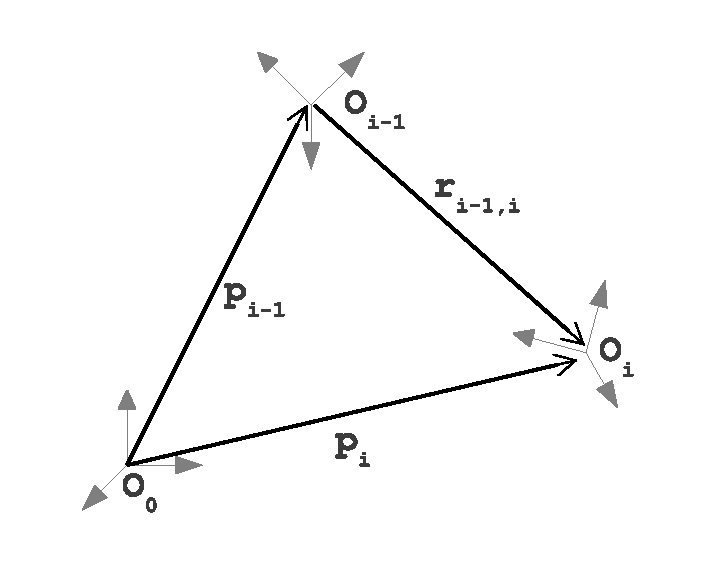
\includegraphics[width=0.6\textwidth]{../figures/link_velocity.eps}
    \caption{Relative position between two origin frames expressed in a common base frame.}
    \label{fig:linkvelocity}
\end{figure}

\subsubsection*{Linear Velocity}
For obtaining the according linear velocity formulation, we can take the first derivative of the above equation \ref{eqn:linkposition}. This yields into:
\begin{eqnarray}
\vec{\dot{p_i}} &=& \vec{\dot{p}_{i-1}} + \vec{R}_{i-1}\vec{\dot{r}_{i-1,i}^{i-1}} + \vec{\omega}_{i-1} \times \vec{R}_{i-1}\vec{r_{i-1,i}^{i-1}} \notag \\
&=& \vec{\dot{p}}_{i-1} 
+ \vec{v}_{i-1,i} + 
\vec{\omega}_{i-1} \times \vec{r}_{i-1,i}
\end{eqnarray}
Hereby, the linear velocity is split into translational velocity $\vec{v}$ and rotational linear velocity $\vec{\omega}_{i-1} \times \vec{r}_{i-1,i}$ between two adjacent links.
\subsubsection*{Angular Velocity}
The angular velocity can be obtained from the rotation matrix composition
\begin{equation}
\vec{R_i} = \vec{R}_{i-1}\vec{R}_{i}^{i-1} \label{eqn:rotationcomp}
\end{equation}
It can be shown in \cite{citeulike:1090825} and \cite{opac-b1129198}, by useful exploiting the skew matrix property, taking the first derivative of equation \ref{eqn:rotationcomp} yields to the angular velocity formulation:
\begin{eqnarray}
\vec{\omega}_i &=& \vec{\omega}_{i-1} + \vec{R}_{i-1} \vec{\omega}_{i-1,i}^{i-1} \notag \\
&=& \vec{\omega}_{i-1} + \vec{\omega}_{i-1,i}
\end{eqnarray}

Furthermore, the relations examined in equation \ref{eqn:linkposition} and \ref{eqn:rotationcomp} differ depending on the type of joint. We have to differentiate the velocity decompositions depending whether we are considering a revolute or prismatic joint:

\subsubsection*{Revolute Joint}
According to the Denavit-Hartenberg Convention (DHC), the axis of rotation is $z$ \cite{hartenberg-1964a}. Hence, the angular velocity simplifies to
\begin{equation}
\vec{\omega}_{i-1,i} = \dot{\theta}_i \vec{z}_{i-1}
\end{equation}
where $\vec{\dot{\theta}}$ denotes the rotational joint speed. Using this, we calculate further the linear velocity:
\begin{equation}
\vec{v}_{i-1,i} = \vec{\omega}_{i-1,i} \times \vec{r}_{i-1,i}
\end{equation}
Once we computed $\vec{\omega}_{i-1,i}$ and $\vec{v}_{i-1,i}$, we finally obtain:
\begin{eqnarray}
\vec{\omega} &=& \vec{\omega}_{i-1} + \dot{\theta}_i \vec{z}_{i-1} \\
\vec{\dot{p}}_i &=& \vec{\dot{p}}_{i-1} + \vec{\omega}_i \times\vec{r}_{i-1,i} 
\end{eqnarray}

\subsubsection*{Prismatic Joint}
Equally to the revolute joints, we have to reconsider the equations of velocity for prismatic joints. Since the prismatic joint has no rotational part, the angular velocity equals zero
\begin{equation}
\vec{\omega}_{i-1,i} = \vec{0}
\end{equation}
Also for prismatic joint, the axis of movement according to DHC is along $z$. The linear velocity results to
\begin{equation}
\vec{v}_{i-1,i} = \dot{d}_i \vec{z}_{i-1}
\end{equation}
The final velocities are computed respectively:
\begin{eqnarray}
\vec{\omega} &=& \vec{\omega}_{i-1} \\
\vec{\dot{p}}_i &=& \vec{\dot{p}}_{i-1} +\dot{d}_i \vec{z}_{i-1} + \vec{\omega}_i \times\vec{r}_{i-1,i} 
\end{eqnarray}

\subsubsection*{Jacobian Calculation}
In equation \ref{eqn:jacobianmap}, we introduced the Jacobian as a mapping between cartesian space and joint space. As we have seen in the former examination, the Jacobian maps rotational and translational velocity towards cartesian velocity. Thus, we can formulate the Jacobian as such:
\begin{equation}
\vec{J} = \begin{pmatrix}
\vec{J}_p \\
\vec{J}_r
\end{pmatrix} = \begin{pmatrix}
\vec{J}_{p_{1}} & \dots & \vec{J}_{p_{n}} \\
\vec{J}_{r_{1}} & \dots & \vec{J}_{r_{n}} \\
\end{pmatrix} \quad ,\textit{with }\vec{J} \in \mathbb{R}^{6 \times n} \label{eqn:jacobiandecomposition}
\end{equation}
where each $\vec{J}_{p_{i}}$,$\vec{J}_{r_{i}}$ describes a 3-dimensional vector, which relates each joint velocity $\dot{q}_i$ to the linear velocity. $\vec{J}_{p_{i}}$ maps $x,y,z$ components of translational velocity into cartesian space. Equally $\vec{J}_{r_{i}}$ relates the orientation in terms of Euler angles $R,P,Y$. 
\begin{equation}
\vec{J}_{p_{i}} = \begin{bmatrix}
J_{p_{i,x}} \\ 
J_{p_{i,y}} \\
J_{p_{i,z}} \\
\end{bmatrix} \quad \quad
\vec{J}_{r_{i}} = \begin{bmatrix}
J_{r_{i,r}} \\ 
J_{r_{i,p}} \\
J_{r_{i,y}} \\
\end{bmatrix}
\end{equation}

In particular the mapping function looks like the following:
\begin{equation}
\begin{bmatrix}
\dot{p}_x \\
\dot{p}_x \\
\dot{p}_x
\end{bmatrix} =
\vec{J}_{p} 
\vec{\dot{q}}  \quad \quad
\begin{bmatrix}
\dot{p}_r \\
\dot{p}_p \\
\dot{p}_y
\end{bmatrix} =
\vec{J}_{r} 
\vec{\dot{q}}
\end{equation}

We can now compute the full Jacobian, taking again the different types of joints into account. We compute each pair of $\vec{J}_{p_{1}}$,$\vec{J}_{r_{1}}$ in equation \ref{eqn:jacobiandecomposition} according to:
\begin{equation}
\vec{J} = 
\begin{pmatrix}
\vec{J}_{p_{1}} \\
\vec{J}_{r_{1}}
\end{pmatrix}=\left\{
\begin{array}{l l}
\begin{pmatrix}
\vec{z}_{i-1} \times (\vec{p}-\vec{p}_{i-1}) \\
\vec{z}_{i-1}
\end{pmatrix} & \textit{for revolute joints} \\[1.7em]
\begin{pmatrix}
\vec{z}_{i-1} \\
\vec{0}
\end{pmatrix} & \textit{for prismatic joints}
\end{array} \right.
\end{equation}
For a detailed and well explained derivation of the above computation, the interested reader is referred to \cite{citeulike:1090825} and \cite{opac-b1129198}. 

\subsection{Jacobian Calculation of Moving Points}
In the previous section, calculated the Jacobian with respect to all related joints along one kinematic chain ending with the tool joint at the tip. Within this calculation, the assumption is taken that all joint position are at the end point of the link. The axis of movement is $Z$. \\
For the purpose of collision avoidance based on a closest point pair, we need the Jacobian in respect of the closest point $p_1$, which varies from the center point on the $z$-axis. As depicted in figure \ref{fig:capsulejacobian}, we need to find a transformation from the Jacobian calculated for frame origin $O_i$ to frame origin $O_{cp}$. This means, we need a mapping from the joint velocities to the linear and angular velocities at point $O_{cp}$. 
\begin{figure}[h!]
  \centering
    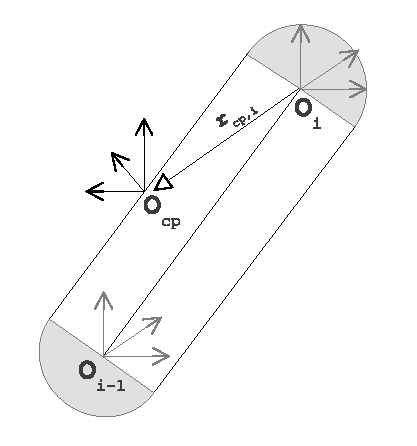
\includegraphics[width=0.3\textwidth]{../figures/capsulejacobian.eps}
    \caption{Jacobian has to be calculated in respect to frame $O_{cp}$. The coordinate frame transformation can be realized with a twist, given the relative transformation $r_{cp,i}$ between $O_i$ and $O_{cp}$. }
    \label{fig:capsulejacobian}
\end{figure}
Since the closest point is part of the capsule, for which origin we can easily calculate the Jacobian, we can treat this as a static transformation. Thus, we can state the following relation:
\begin{eqnarray}
\vec{\dot{p}_{cp}} &=& \vec{\dot{p}_i} + \vec{\omega_i} \times \vec{r}_{cp,i}  \notag \\
\vec{\omega_{cp}} &=& \vec{\omega_i}
\end{eqnarray}
By utilizing the skew-symmetric operator $S(\bullet)$, we can write the above relation in matrix notation. 
\begin{equation}
\begin{pmatrix}
\vec{\dot{p}_{cp}} \\
\vec{\omega_{cp}}
\end{pmatrix}  = 
\begin{pmatrix}
\vec{I} & -\vec{S}(\vec{r}_{cp,i}) \\
\vec{0} & \vec{I}
\end{pmatrix} 
\begin{pmatrix}
\vec{\dot{p}_{i}} \\
\vec{\omega_{i}}
\end{pmatrix} \label{eqn:twist}
\end{equation} 
This results in a twist computation as the linear projection now describes a $\mathbb{R}^{6\times6}$ matrix. We can use this formulation in order to obtain the Jacobian at point $O_{cp}$. If we substitute $\vec{\dot{p}_{cp}}$ and $\vec{\omega_{cp}}$ with the Jacobian mapping function, equation \ref{eqn:twist} yields
\begin{eqnarray}
\begin{pmatrix}
\vec{\dot{p}_{cp}} \\
\vec{\omega_{cp}}
\end{pmatrix}  &=& 
\begin{pmatrix}
\vec{I} & -\vec{S}(\vec{r}_{cp,i}) \\
\vec{0} & \vec{I}
\end{pmatrix} 
\begin{pmatrix}
\vec{\dot{p}_{i}} \\
\vec{\omega_{i}}
\end{pmatrix} \notag \\ [0.7em]
\vec{J}(\vec{p}_{cp},\vec{q})\vec{\dot{q}} &=& 
\begin{pmatrix}
\vec{I} & -\vec{S}(\vec{r}_{cp,i}) \\
\vec{0} & \vec{I}
\end{pmatrix} 
\vec{J}(\vec{p}_{i},\vec{q})\vec{\dot{q}}
\notag \\ [0.7em]
\vec{J}(\vec{p}_{cp},\vec{q}) &=& 
\begin{pmatrix}
\vec{I} & -\vec{S}(\vec{r}_{cp,i}) \\
\vec{0} & \vec{I}
\end{pmatrix} 
\vec{J}(\vec{p}_{i},\vec{q}) \label{eqn:solvejaccp}
\end{eqnarray}

With the above formulation, we can calculate the Jacobian at any point of the capsule. Most kinematic or dynamic libraries provide already the capability of computing the Jacobian along the kinematic chain up to the end effector position. Thus, for every update of the solver, we have to compute the relative transformation $\vec{r}_{cp,i}$ and obtain the according Jacobian based on equation \ref{eqn:solvejaccp}. 